% --------------------------------------------------
% DISCUSSION: ECONOMIC AND MANAGERIAL IMPLICATIONS
% --------------------------------------------------
\section{Discussion: Economic and Managerial Implications}
\label{sec:discussion}

The Cox model results establish that abandonment in Grand Tours is systematically associated with rider-level proxies for continuation costs and race-level proxies for incentives. This section draws out the implications of these findings for three audiences: team management, race organisers, and the broader economics-of-sports literature.

\subsection{Implications for Team Management}

Professional cycling teams are, in the framework of \textcite{blair2012sports}, profit-maximising firms that must allocate scarce resources (rider effort, support staff, and budget) across a calendar of events. The finding that historical DNF rate is the strongest predictor of abandonment, and that its effect is amplified for GC contenders (HR $= 2.280$ vs.\ $1.472$ for non-GC riders), has direct implications for roster selection and race strategy.

First, consider \emph{roster selection}. When a team chooses which eight or nine riders to send to a Grand Tour, it faces a portfolio problem: each rider brings expected performance but also an expected probability of attrition. The hazard model suggests that a rider's past DNF rate is a strong signal of future abandonment risk. A team building a GC campaign around a fragile leader (one with a high historical DNF rate) should therefore allocate additional domestique resources as insurance, or consider whether the expected return from that rider's GC bid justifies the elevated risk of losing the team's primary investment mid-race. This connects to the contract-design literature in professional sports: \textcite{krautmann2002contracts} show that contract length in Major League Baseball reflects expected future performance, and an analogous logic applies in cycling, where a rider's abandonment history should be priced into contract negotiations.

Second, consider \emph{within-race resource allocation}. The time-varying model shows that mountain stages significantly raise daily abandonment hazard. A team directeur sportif (DS) who knows this can adjust domestique deployment accordingly: concentrate support on mountain stages where the GC contender is most vulnerable, and allow domestiques more freedom on flat stages where abandonment risk is low. This is a form of dynamic resource allocation under uncertainty, where the hazard model provides the signal and the DS acts as the firm's real-time manager. The finding that the GC contender effect loses significance once stage-type controls are added (Section~\ref{sec:results}) reinforces this interpretation: it is not GC status per se that drives abandonment, but rather the interaction between GC contenders and the specific stages that test them most severely.

Third, there is a \emph{principal-agent dimension} to the abandonment decision. The team (principal) may want the rider (agent) to continue---for team UCI points, sponsor visibility, and contractual obligations---even when the rider's private assessment is that the cost of continuing exceeds his personal expected benefit. Conversely, a team may instruct a rider to abandon strategically to preserve him for future events, even if the rider would prefer to continue for personal pride or individual prize money. This tension is not directly observable in the data, but it is consistent with the finding that GC contenders have higher abandonment hazard: these are precisely the riders for whom the team's strategic interest in withdrawal (once GC contention is lost) is strongest.

Figure~\ref{fig:gc_vs_nonGC} illustrates the heterogeneity in abandonment determinants across rider roles. The sharply different hazard ratio magnitudes for previous DNF rate between GC contenders and non-GC riders visually reinforce the argument that team management must differentiate its abandonment strategy by rider type.

\begin{figure}[H]
    \centering
    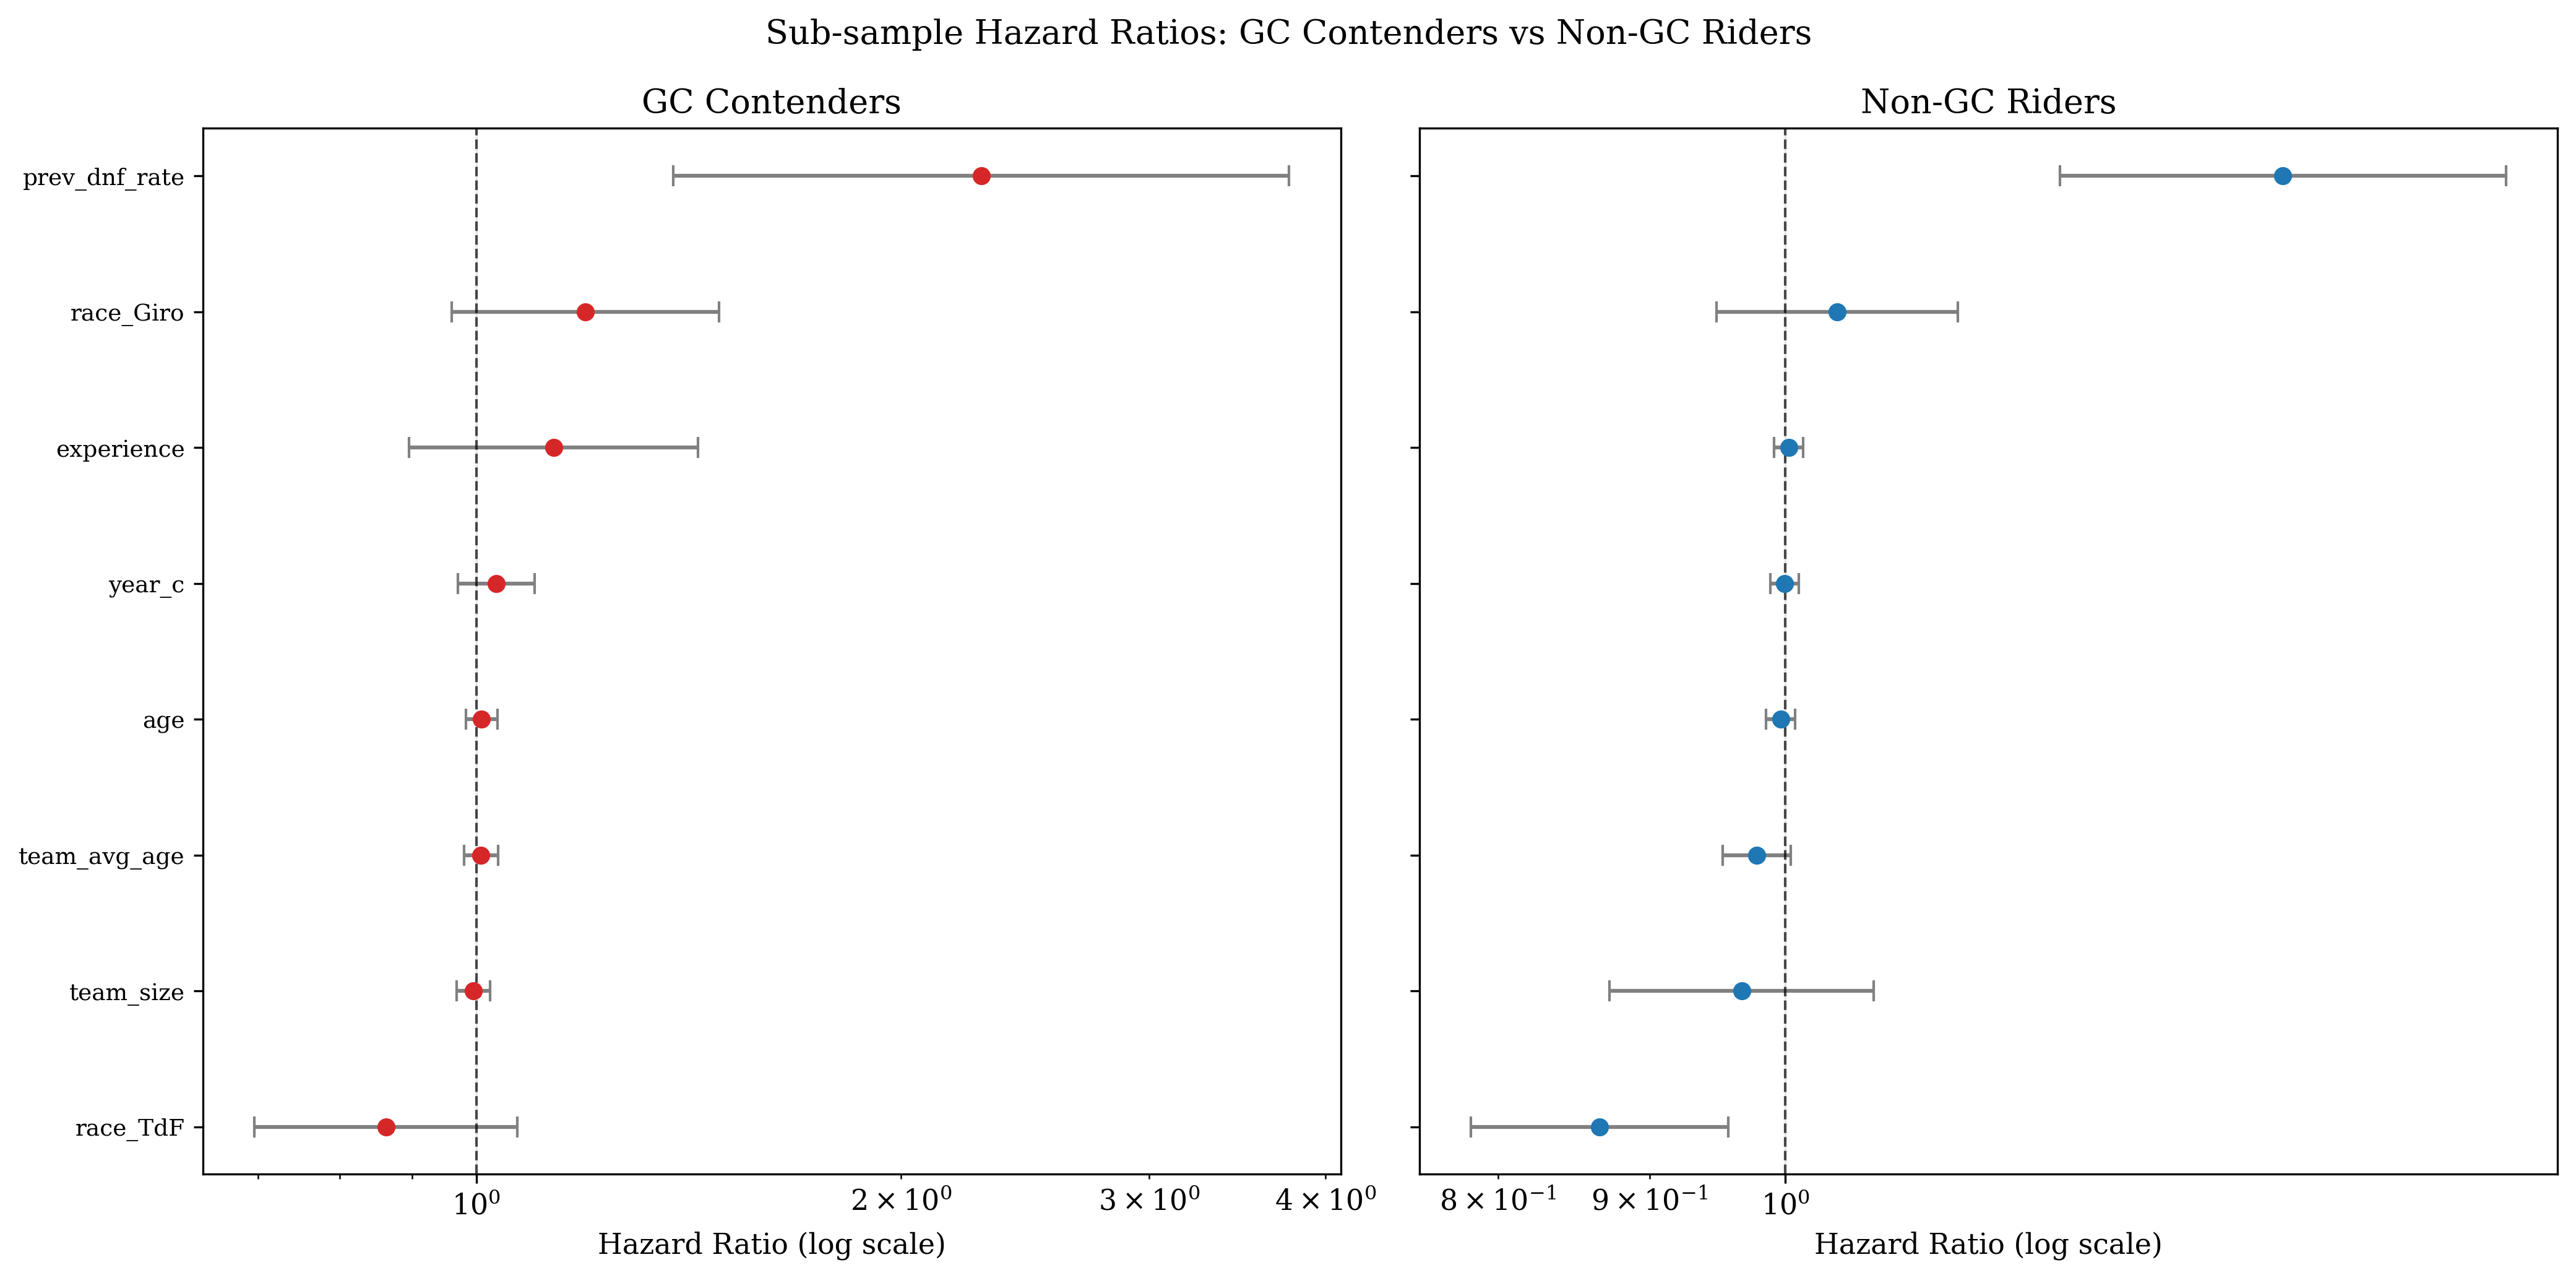
\includegraphics[width=0.80\linewidth]{Afsnit/Billeder/fig7_gc_vs_nonGC_hazard_ratios.png}
    \caption{Hazard ratios from separate Cox PH models for GC contenders (left panel) and non-GC riders (right panel). The previous DNF rate effect is substantially larger for GC contenders, while the Tour de France protective effect is significant only for non-GC riders.}
    \label{fig:gc_vs_nonGC}
\end{figure}

\subsection{Implications for Race Organisers and League-Level Design}

From the perspective of a race organiser such as ASO (Amaury Sport Organisation, which runs the Tour de France), rider abandonment is not merely a sporting outcome; it is a product-quality issue. A Grand Tour where a large share of the field abandons delivers a diminished spectacle to viewers: fewer riders in the peloton, fewer competitive battles in the final week, and a higher probability that marquee names disappear from the broadcast. \textcite{courty2003ticketresale} shows that spectators value ex-ante uncertainty of outcome; when a GC favourite abandons, that uncertainty is resolved prematurely, reducing the entertainment value of remaining stages. The finding that the Tour de France has the lowest abandonment rate is reassuring for ASO, but it also suggests that the Giro and Vuelta organisers face a competitive disadvantage: lower event prestige leads to higher attrition, which in turn may further reduce media interest---a potential negative feedback loop.

The mountain-stage effect has direct implications for \emph{route design}. Race organisers choose where to place mountain stages, how many consecutive mountain days to schedule, and how severe the climbs should be. The hazard model suggests that mountain stages raise abandonment risk, which means that a route with five consecutive mountain stages in the third week (as the Giro sometimes schedules) will produce more abandonments than a route that spreads the mountains more evenly. Whether this is desirable depends on the organiser's objective function: more attrition may create drama (the strongest rider survives), but it may also thin the field to the point where the race loses its visual and competitive appeal. This trade-off between selectivity and spectacle is a classic design problem in the economics of sporting contests \parencite{szymanski2003economicdesign}.

The counterfactual analysis in Figure~\ref{fig:counterfactual} illustrates the concrete consequences of GC contender abandonment for race outcomes. The wide range of counterfactual finishing positions shows that some abandoned GC contenders would have finished inside the top 20, redistributing UCI ranking points and prize money among the remaining riders. When a rider who would have finished in the top 10 abandons, the final GC standings change in ways that affect future contract negotiations and team selection, because the GC classification serves as a key performance signal in the cycling labour market \parencite{boeri2008italianjob}. This means that the observable GC standings are, to some degree, an artifact of who chose or was forced to abandon rather than a pure measure of rider quality.

\begin{figure}[H]
    \centering
    \includegraphics[width=0.75\linewidth]{Afsnit/Billeder/fig8_gc_counterfactual.png}
    \caption{Counterfactual GC finishing positions for abandoned GC contenders (2010--2025). Each bar represents a rider who abandoned; the counterfactual position is imputed by inserting the rider's last observed cumulative time gap into the actual final GC standings. The wide range illustrates the heterogeneity of abandonment decisions and their consequences for the final classification.}
    \label{fig:counterfactual}
\end{figure}

At the league level, the UCI (Union Cycliste Internationale) has an interest in the overall health of Grand Tour racing. If abandonment is driven partly by economic incentives (riders and teams withdrawing when the expected return falls below the expected cost), then the UCI's own policies affect attrition. The distribution of UCI ranking points across races, the prize-money structures, and the rules governing team selection for Grand Tours all shape the incentive environment. The finding that the Tour de France has lower abandonment hazard, consistent with its higher economic value, implies that making the Giro and Vuelta more commercially attractive (through better broadcasting deals, higher prize money, or more UCI points) could reduce their abandonment rates. This is a testable policy prediction that follows directly from the event-value hypothesis.

\subsection{Connections to Broader Sports Economics Issues}

The analysis in this paper touches on several themes from the broader sports economics literature that deserve brief discussion.

\emph{Doping and anti-doping policy.} The sample period (2010--2025) falls entirely within the biological passport era, during which anti-doping enforcement in cycling intensified significantly. Doping reduces the physical cost of continuation by allowing riders to recover faster and sustain higher power outputs over three weeks. The tightening of anti-doping controls therefore raises the ``clean'' cost of continuation, potentially increasing abandonment rates for riders who previously relied on pharmaceutical assistance. While the year trend in the model is not significant, the interaction between anti-doping policy and abandonment behaviour is a plausible channel that future research could explore, for instance by comparing abandonment rates before and after major policy changes.

\emph{Betting markets and information asymmetry.} Grand Tour stage betting is a growing market, and rider abandonment creates a potentially exploitable information asymmetry. Team staff, soigneurs, and the rider himself know before a stage start whether the rider is likely to abandon, information that is not available to the betting market until the rider actually climbs off his bike. \textcite{duggan2002sumo} document how strategic behaviour in sumo wrestling can be inferred from statistical patterns in outcomes, and the same logic applies here: if abandonment is partly strategic (as the GC contender results suggest), then the timing of abandonment may carry information that is valuable to insiders. This suggests that abandonment data could be useful for monitoring suspicious betting patterns.
